% !TEX root = ../memorianueva.tex
% Appendix A

% Este anexo es solo de figuras: sin estos ajustes LaTeX exige un mínimo de
% texto por página y deja una sola imagen por hoja, con mucho espacio en blanco.
\renewcommand{\topfraction}{0.95}
\renewcommand{\bottomfraction}{0.95}
\renewcommand{\textfraction}{0.05}
\renewcommand{\floatpagefraction}{0.85}
\setcounter{topnumber}{4}
\setcounter{bottomnumber}{4}
\setcounter{totalnumber}{6}

\chapter{Capturas del sistema en operación}
\label{AppendixA}

En este anexo se incluyen las imágenes reales del sistema en funcionamiento: el ticket generado y las vistas del panel web de control.

\section{Ticket impreso}

\begin{figure}[htbp]
    \centering
    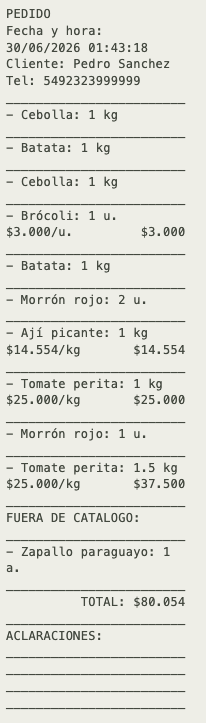
\includegraphics[height=0.52\textheight]{Figures/ticket_impreso.png}
    \caption{Ticket real generado por el sistema e impreso en el comercio.}
    \label{fig:ticket_real}
\end{figure}

\FloatBarrier

\section{Panel web de control}

\begin{figure}[htbp]
    \centering
    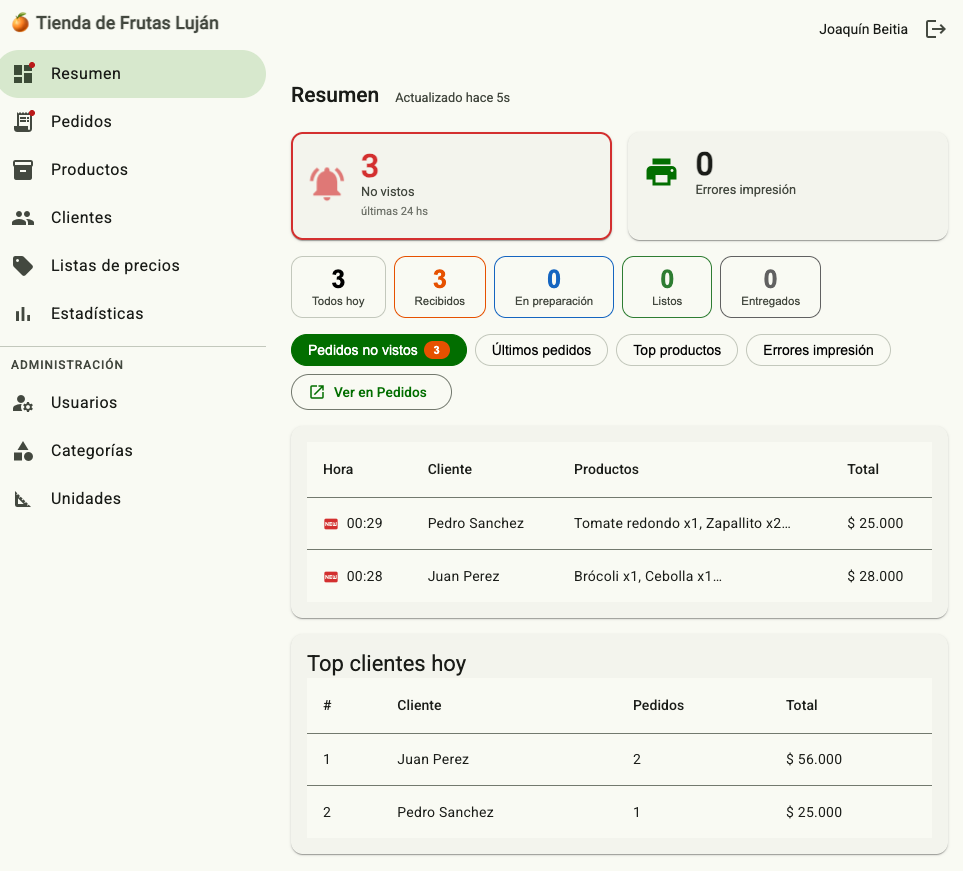
\includegraphics[width=0.82\textwidth]{Figures/panel_dashboard.png}
    \caption{Tablero principal del panel de control.}
    \label{fig:panel_tablero}
\end{figure}

\begin{figure}[htbp]
    \centering
    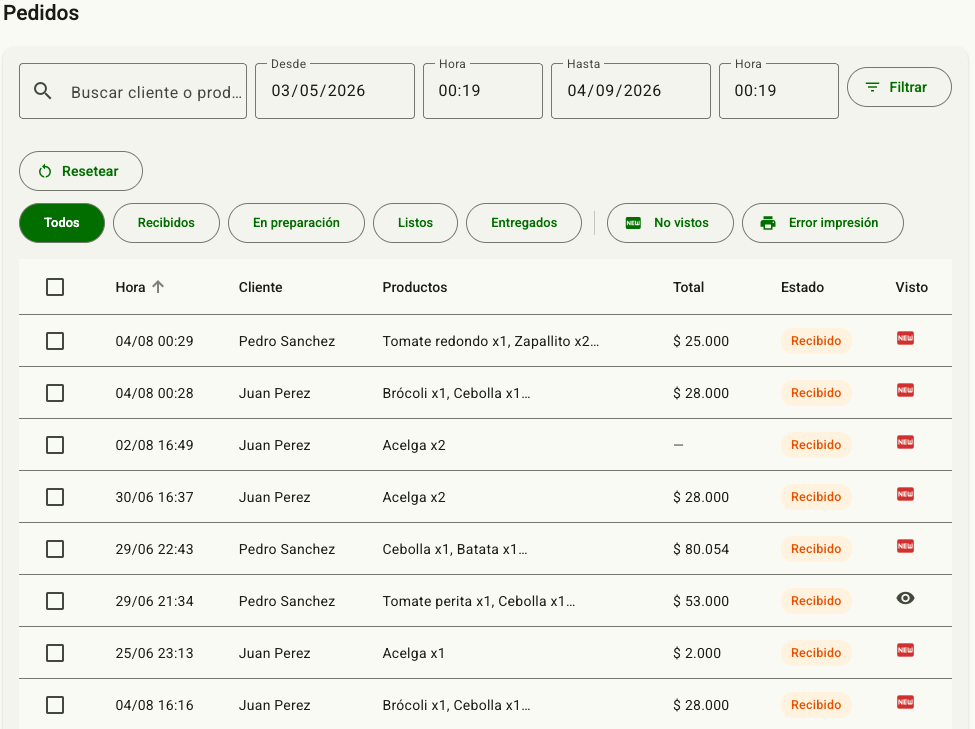
\includegraphics[width=0.82\textwidth]{Figures/panel_pedidos.png}
    \caption{Listado de pedidos con sus filtros de búsqueda.}
    \label{fig:panel_pedidos}
\end{figure}

\begin{figure}[htbp]
    \centering
    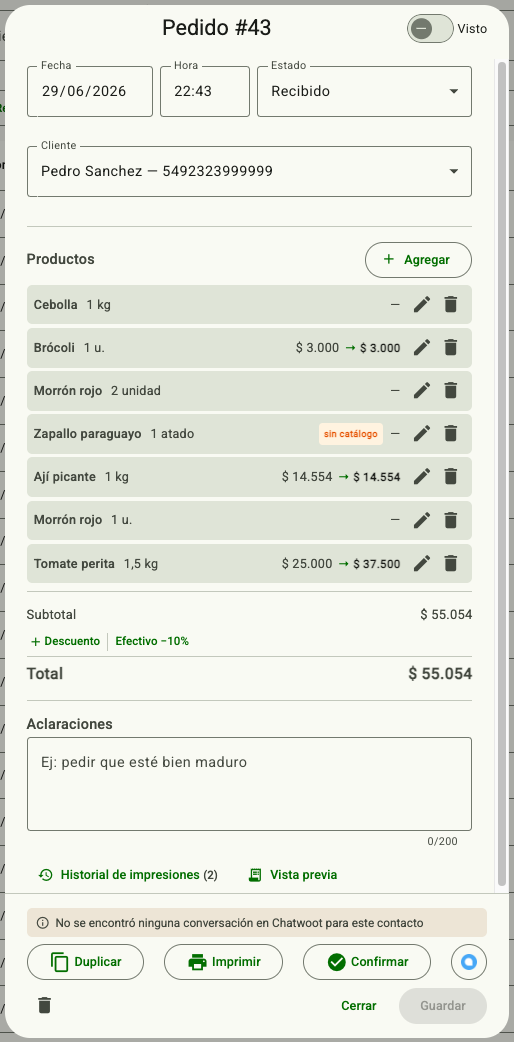
\includegraphics[width=0.4\textwidth]{Figures/panel_detalle_pedido.png}
    \caption{Detalle de un pedido, con edición de ítems y acceso al mensaje original.}
    \label{fig:panel_detalle}
\end{figure}

\begin{figure}[htbp]
    \centering
    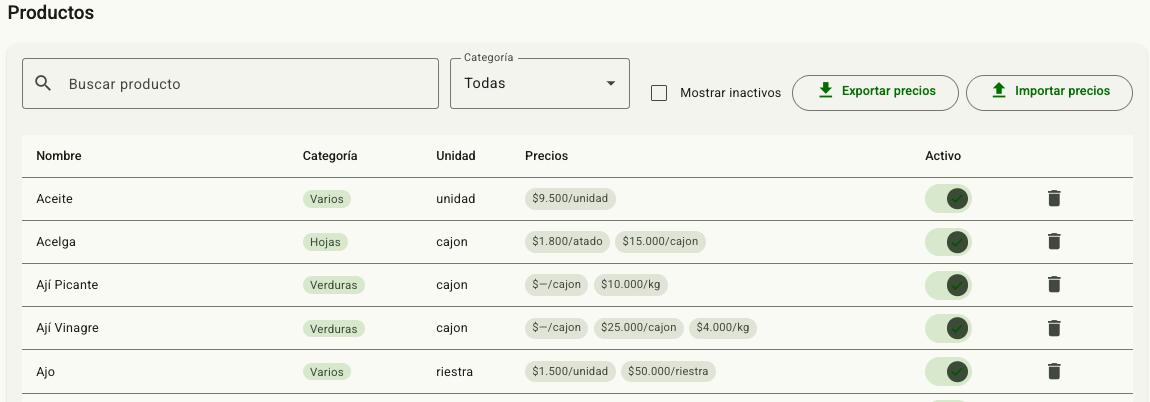
\includegraphics[width=\textwidth]{Figures/panel_productos.png}
    \caption{Administración del catálogo de productos.}
    \label{fig:panel_catalogo}
\end{figure}

\begin{figure}[htbp]
    \centering
    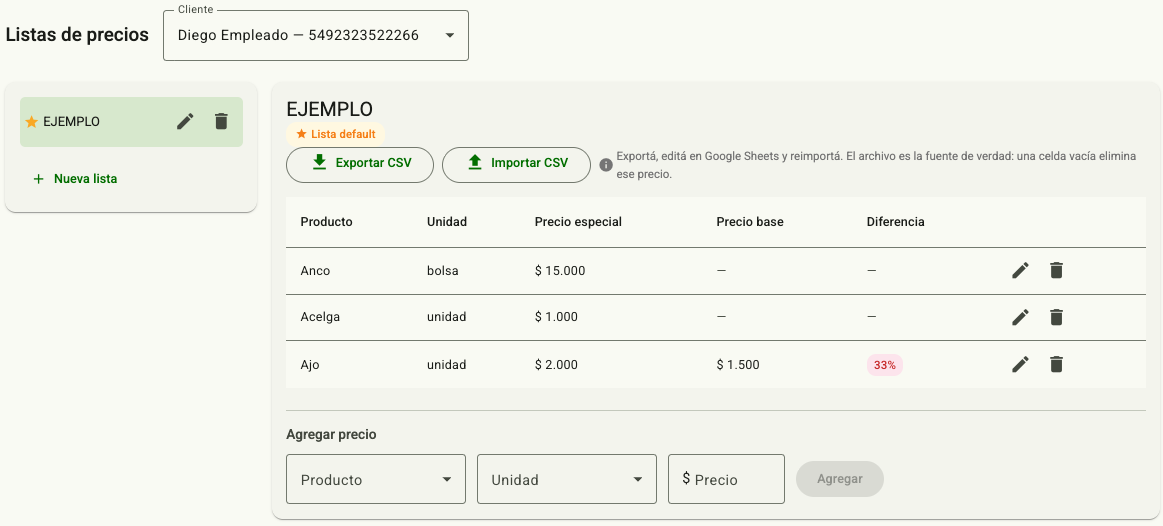
\includegraphics[width=\textwidth]{Figures/panel_listas_precios.png}
    \caption{Administración de las listas de precios de un cliente.}
    \label{fig:panel_precios}
\end{figure}

\begin{figure}[htbp]
    \centering
    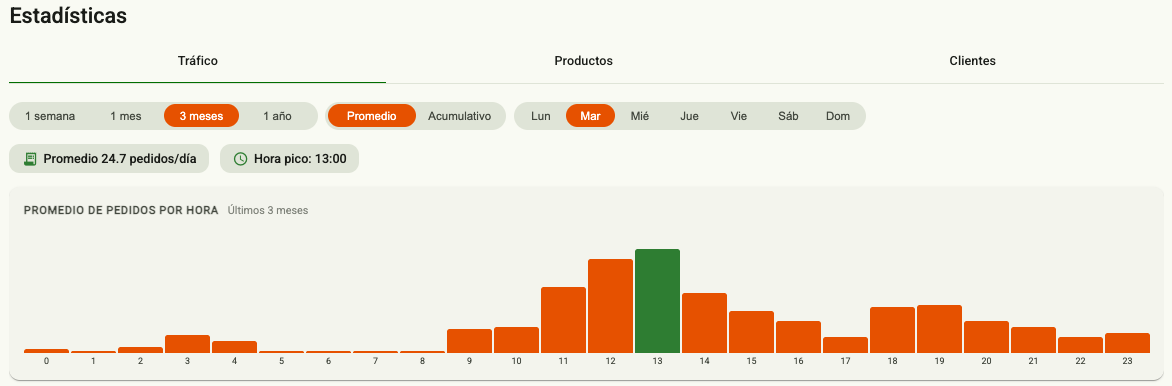
\includegraphics[width=\textwidth]{Figures/panel_estadisticas.png}
    \caption{Vista de métricas de operación del comercio.}
    \label{fig:panel_metricas}
\end{figure}

\FloatBarrier
